
\chapter{Grafos gerados referentes ao \emph{ResourceManager}}
\label{chap:ApendA}

A seguir encontram-se uma breve explicação e as figuras geradas pelo segundo método empregado na etapa de estudo da arquitetura do \emph{framework}.

A pertinência das figuras é validada por elas descreverem todos os caminhos possíveis que dada interface pode tomar. O fluxo do caso perfeito seria iniciado com o recebimento de um novo \emph{job} pelo \emph{ResourceManager}. Para que o \emph{job} possa ser iniciado alguns pré-requisitos devem ser satisfeitos. É a partir desse ponto que as figuras entram em cena.

Para que uma aplicação seja iniciada, primeiramente é criado um \emph{AppAttempt}. O \emph{AppAttempt} é literalmente uma tentativa de aplicação, pela qual o \emph{ResourceManager} tentará alocar os recursos necessários (\emph{Node e Container}) para que essa aplicação seja realmente criada e submetida ao cluster. Durante o processo do \emph{RMAppAttempt} o \emph{ResourceManager} irá tentar alocar um ou mais \emph{RMContainers} bem como \emph{RMNodes} para que a aplicação tenha recursos suficientes para sua execução. Após os recursos necessários terem sido alocados com sucesso, a aplicação passa para o status de \emph{RMApp} e é submetida ao cluster.

%IMPORTANTE: Se precisar usar alguma seção ou subseção dentro dos apêndices ou
%anexos, utilizar o comando \tocless para não adicionar no Sumário
%Exemplos: 
% \tocless\section{Histórico}
% \tocless\subsection{Detalhes}
%\tocless\section{teste}
%Este é um teste de seção dentro do apêndice

\begin{figure}[hbtn]
   \centering
   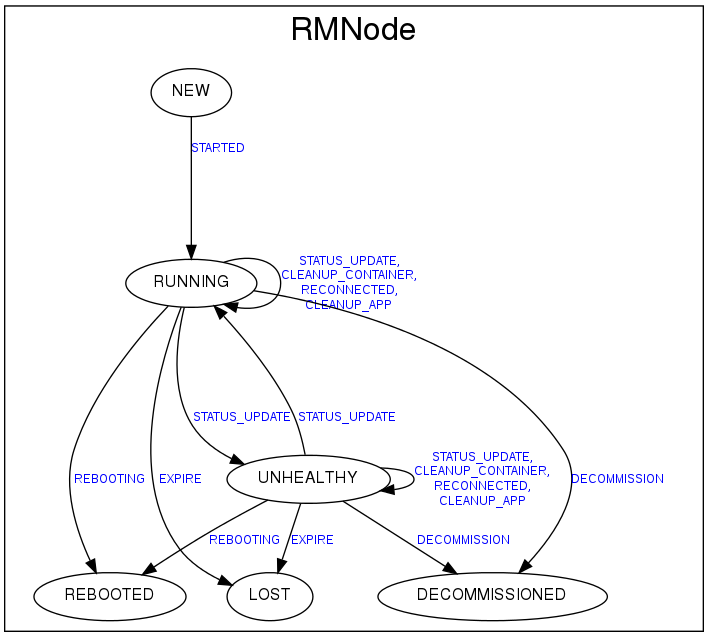
\includegraphics[width=12cm]{figuras/Figura05-RMNode.png}
   \caption{Máquina de estados do RMNode}
   \label{fig:RMNode}
\end{figure}

\begin{figure}[hbtn]
   \centering
   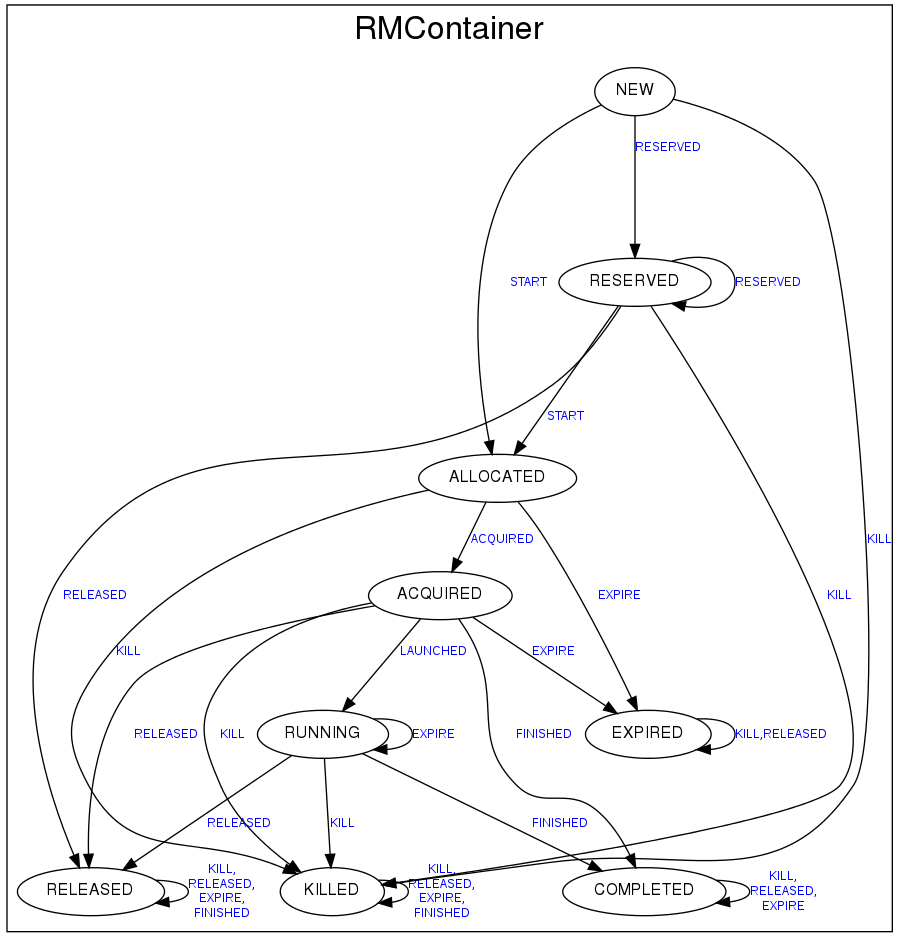
\includegraphics[width=15cm]{figuras/Figura03-RMContainer.png}
   \caption{Máquina de estados do RMContainer}
   \label{fig:RMContainer}
\end{figure}

\begin{figure}[hbtn]
   \centering
   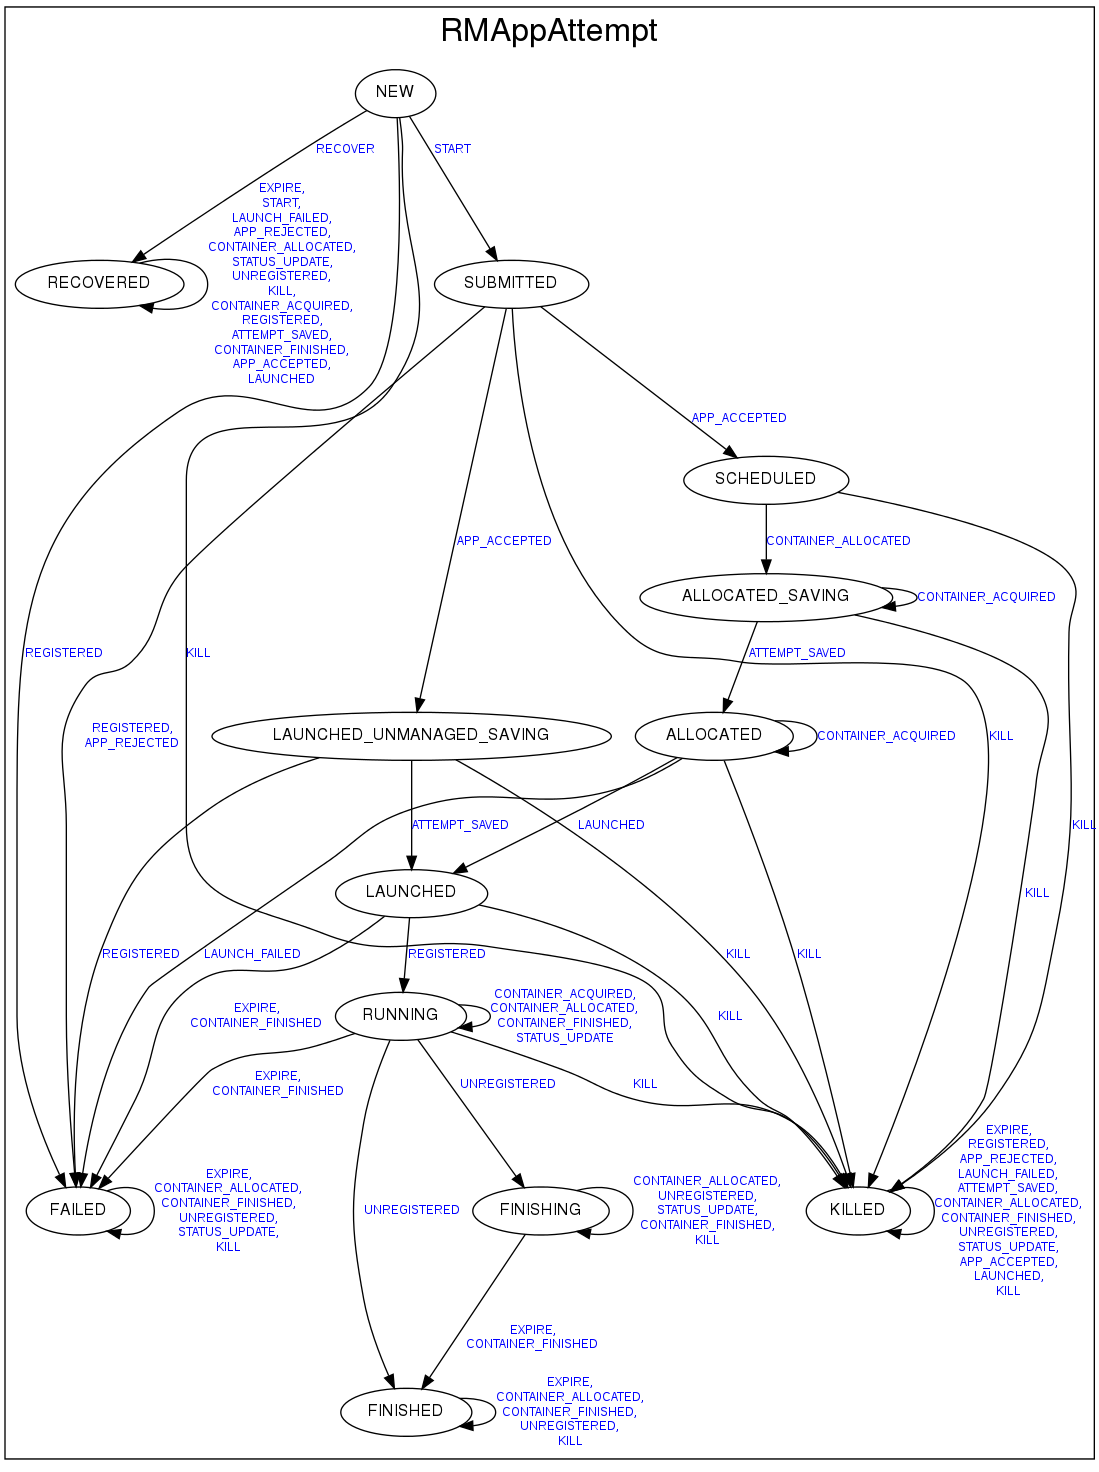
\includegraphics[width=15cm]{figuras/Figura02-RMAppAttempt.png}
   \caption{Máquina de estados do RMAppAttempt}
   \label{fig:RMAppAttempt}
\end{figure}

\begin{figure}[hbtn]
   \centering
   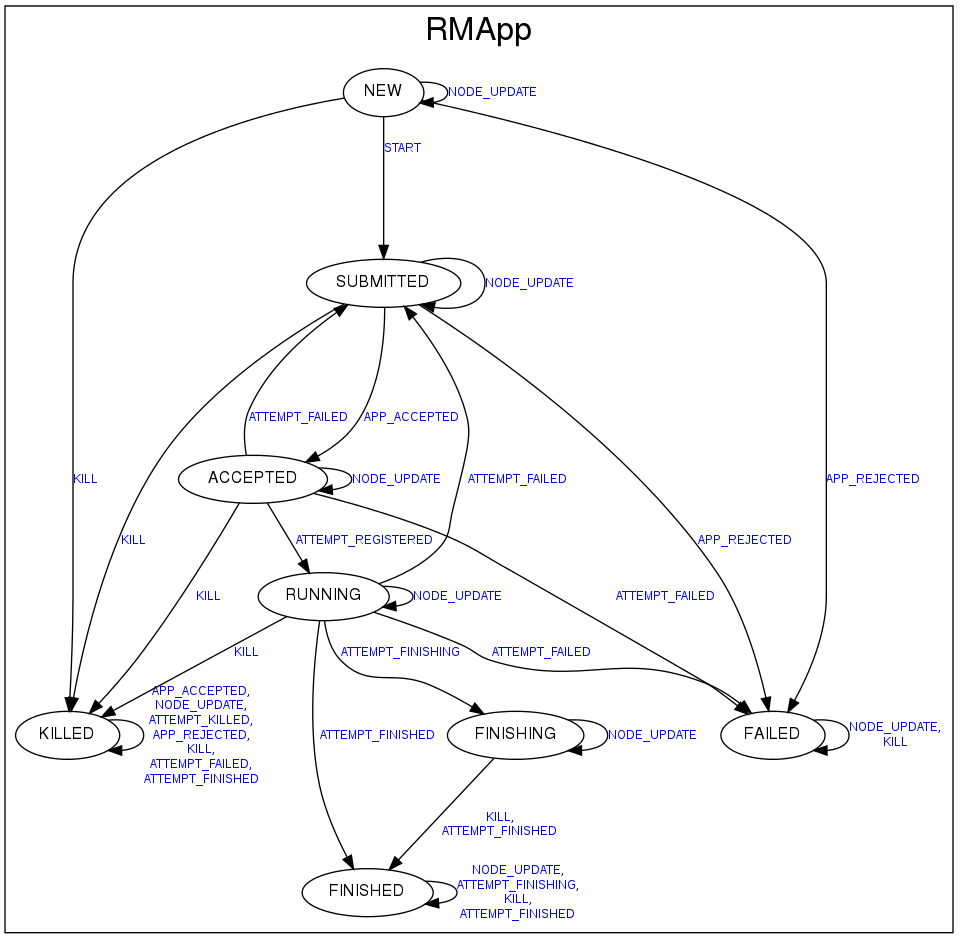
\includegraphics[width=15cm]{figuras/Figura04-RMApp.png}
   \caption{Máquina de estados do RMApp}
   \label{fig:RMApp}
\end{figure}